\subsection{Duomenų dalijimo klasė}
\label{subsec:data_splitter}

Duomenų dalijimo (\texttt{DataSplitter}) klasės veikimas (žr.~\ref{fig:data_splitter_class} pav.):

\begin{enumerate}
    \item Klasė priima jau sutvarkytus požymius ir klases iš \texttt{DataCleaner} klasės.
    \item Atliekamas pirmasis padalijimas: $80\ \%$ duomenų skiriama mokymo ir validavimo aibėms, $20\ \%$ – testavimo aibei.
    \item Atliekamas antrasis padalijimas: iš pirmo žingsnio gautų $80\ \%$ duomenų, $80\ \%$ skiriama mokymui ir $20\ \%$ – validavimui.
    \item Galutinis santykis: $64\ \%$ mokymo, $16\ \%$ validavimo, $20\ \%$ testavimo.
    \item Atspausdinamas kiekvienos aibės dydis ir klasių pasiskirstymas jose.
\end{enumerate}

\begin{figure}[H]
    \centering
    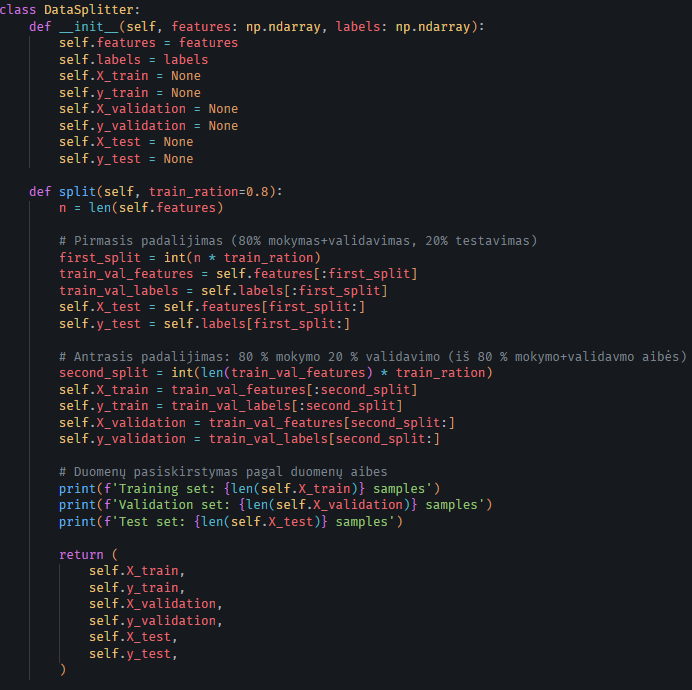
\includegraphics[width=0.75\linewidth]{2Lab/overleaf/images/DataSplitter_Class.png}
    \caption{Duomenų dalijimo klasės kodas}
    \label{fig:data_splitter_class}
\end{figure}